\section{\Large PROBLEM SET 2}
\subsection{PROBLEM 1}
\textit{Define orbit initial conditions and make sure you can propagate the orbit of the satellite over multiple orbits using either a Keplerian propagator or a numerical integration scheme (see AA279A material). Best would be to use a numerical integrator, so that you can later try to feed the same environmental forces for orbit propagation which are applied for attitude propagation (very cool!).}

From the science users' handbook, we obtain the following orbital elements \cite{NISARHandbook}.

\begin{table}[H]
\begin{tabular}{lllllll}
\textbf{OE} & \textit{a} & \textit{e} & \textit{i} & \textit{$\Omega$} & \textit{$\omega$} & \textit{$\nu$} \\ \hline
\textbf{Value} & 7125.48662 km & 0.0011650 & 98.40508$\degree$ & -19.61601$\degree$ & 89.99764$\degree$ & -89.99818$\degree$
\end{tabular}
\end{table}

We convert these using a MATLAB function into ECI coordinates that can be fed into a numerical orbital propagator. Notice that we first convert the orbital elements a, e, and $\nu$ into perifocal (PQW) coordinates, using a and e to find the semi-latus rectum and a, e, and $\nu$ to find the distance to the central body (Earth). Then, we perform a series of rotations on these coordinates parameterized by $\omega$, i, and $\Omega$ to obtain new coordinates in the ECI frame.

\lstinputlisting{src/oe2eci.m}

Then, we can numerically propagate in MATLAB using \texttt{ode113} using a function that computes the time derivative of the ECI state. This is accomplished simply by setting the time derivative of position equal to the velocity portion of the state and setting the time derivative of velocity equal to an acceleration computed using the law of universal gravitation. Note that while our propagator does not include disturbance forces, it will be easy to incorporate these later. See the appendix corresponding to Problem Set 2 for application of \texttt{ode113}.

\lstinputlisting{src/orbitSimple.m}

Now, we plot the trajectory for one orbit in Figure \ref{fig:simple_propagator}. Plotting multiple orbits (for example, over 12 days) yields the same plot, as \texttt{ode113} is very stable for this application.

\begin{figure}[H]
\centering
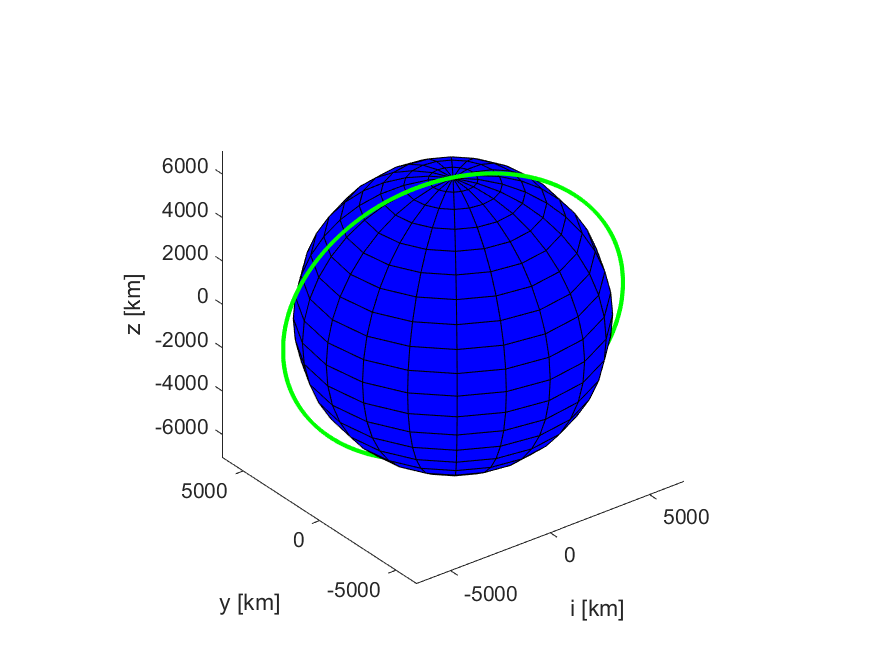
\includegraphics[scale=0.7]{Images/ps2_problem1.png}
\caption{A single orbit for NISAR in ECI coordinates (no perturbations)}
\label{fig:simple_propagator}
\end{figure}


\subsection{PROBLEM 2}
\textit{In general the body axes are not the principal axes. Identify principal axes through the eigenvector/eigenvalue problem discussed in class and compute the rotation matrix from body to principal axes.}

The unit vectors of the principal axes with respect to the body axes ($\Vec{e}_i$) and the inertia tensor in the principal axes ($I_i$) can be found by taking the eigenvalue decomposition of the inertia tensor in the body axis. This can be seen in the two equations below.

\begin{equation*}
    I_i \cdot \Vec{e}_i = I_i \cdot \Vec{I}_{body} \\ \hspace{1cm} i = x, y, z
\end{equation*}

\begin{align*}
\Vec{I}_{principal} &= 
    \begin{bmatrix}
    I_x & 0 & 0 \\
    0 & I_y & 0 \\
    0 & 0 & I_z 
    \end{bmatrix}
= 
\qty[parse-numbers = false]{
    \begin{bmatrix}
    7707.07 & 0 & 0 \\
    0 & 14563.2 & 0 \\
    0 & 0 & 18050.4 
    \end{bmatrix}
}{\kilogram\metre\squared}
\end{align*}

We follow convention $I_z > I_y > I_x$ for defining principal axes.

The unit vectors of the principal axes ($\Vec{e}_i$) can then be used to find the rotation matrix ($\Vec{R}$), as shown below.

\begin{align*}
\Vec{R} &= 
    \begin{bmatrix}
    \Vec{e}_x & \Vec{e}_y & \Vec{e}_z 
    \end{bmatrix}
= 
    \begin{bmatrix}
    -0.06278 & -0.99803 & 0 \\
    0 & 0 & 1 \\
    -0.99803 & 0.06278 & 0 
    \end{bmatrix} \\
    \Vec{I}_{body} &= \Vec{R} \Vec{I}_{principal} \Vec{R}^{\intercal}
\end{align*}


\subsection{PROBLEM 3}
\textit{At this stage you should have a simple 3D model of your spacecraft including geometry and mass properties of each element. This includes at least two coordinate systems, body and principal axes respectively, and the direction cosine matrix between them. Plot axes of triads in 3D superimposed to spacecraft 3D model.}

\begin{figure}[H]
\centering
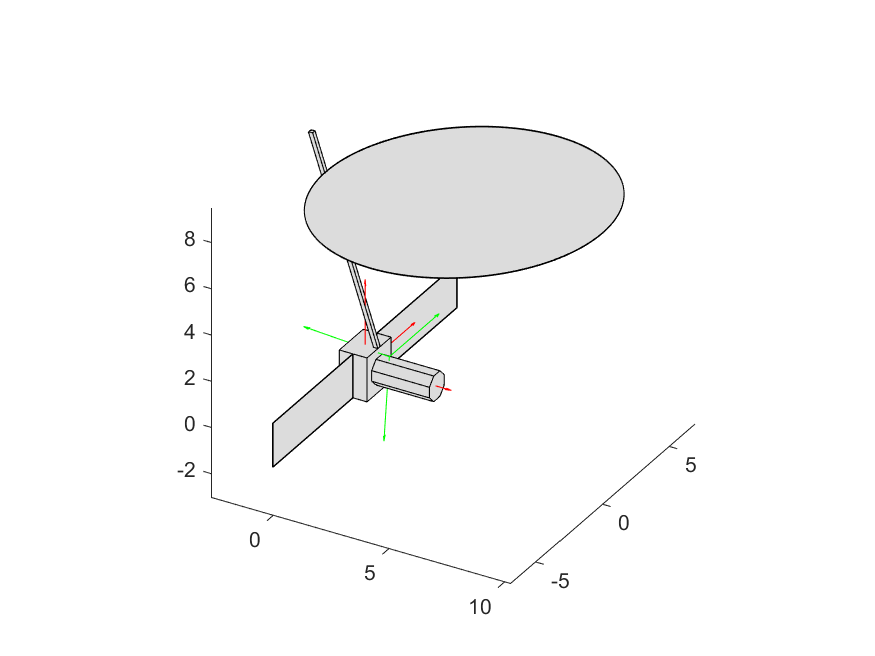
\includegraphics[scale=0.7]{Images/ps2_model.png}
\caption{Principal axes at center of mass (green) and body axes at origin (red)}
\label{fig:ps2_model}
\end{figure}


\subsection{PROBLEM 4}
\textit{Program Euler equations in principal axes (e.g. in Matlab/Simulink). No external torques.}

We use the following equations with zero external moments ($M_{x}, M_{y}, M_{z} = 0$).

\begin{align*}
    I_{x} \Dot{\omega}_{x} + (I_{z} - I_{y}) \omega_{y} \omega_{z} &= M_{x} \\
    I_{y} \Dot{\omega}_{y} + (I_{x} - I_{z}) \omega_{z} \omega_{x} &= M_{y} \\
    I_{z} \Dot{\omega}_{z} + (I_{y} - I_{x}) \omega_{x} \omega_{y} &= M_{z}
\end{align*}

\lstinputlisting{src/eulerEquation.m}


\subsection{PROBLEM 5}
\textit{Numerically integrate Euler equations from arbitrary initial conditions ($\omega<\qty{10}{\degree/\second}$, $\omega_{i}\neq0$). Multiple attitude revolutions.}

We choose arbitrary initial conditions $\omega_{x} = \qty{8}{\degree\per\second}$, $\omega_{y} = \qty{4}{\degree\per\second}$, and $\omega_{z} = \qty{6}{\degree\per\second}$. The results of numerical integration using \texttt{ode113} are shown in Figure \ref{fig:ps2_euler_equations}.

\begin{figure}[H]
\centering
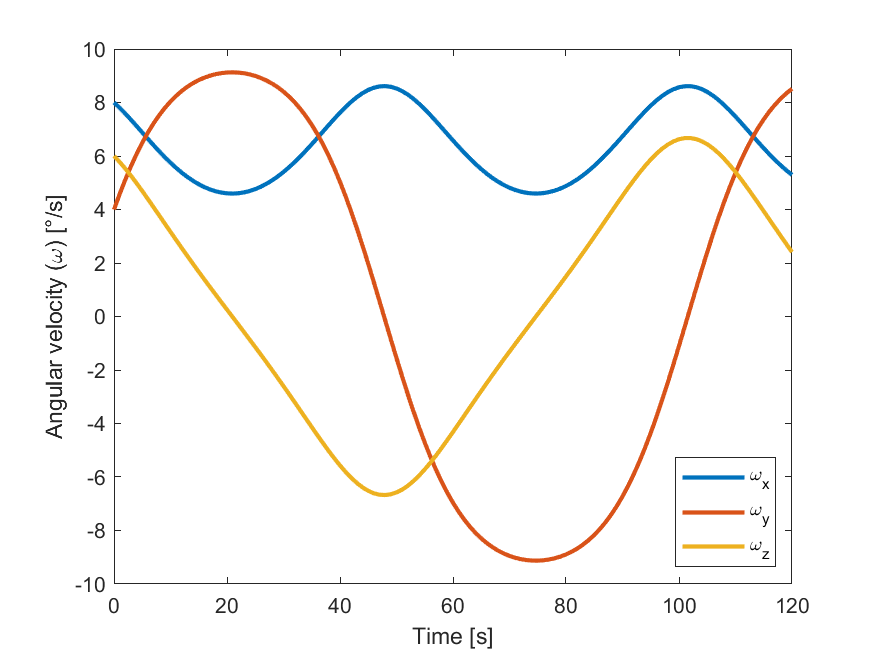
\includegraphics[scale=0.6]{Images/ps2_euler_equations.png}
\caption{Results from numerical integration of Euler equations}
\label{fig:ps2_euler_equations}
\end{figure}


\subsection{PROBLEM 6}
\textit{Plot rotational kinetic energy and momentum ellipsoids in 3D (axis equal) corresponding to chosen initial conditions. Verify that semi-axis of ellipsoids corresponds to theoretical values.}

For the energy ellipsoid, we compute our surface using rotational kinetic energy based on initial conditions and principal axes inertia tensor.

\begin{align*}
    &2T = \omega_{x}^{2} I_{x} + \omega_{y}^{2} I_{y} + \omega_{z}^{2} I_{z} \\
    &\frac{\omega_{x}^{2}}{2T/I_{x}} + \frac{\omega_{y}^{2}}{2T/I_{y}} + \frac{\omega_{z}^{2}}{2T/I_{z}} = 1
\end{align*}

For the given initial conditions, we get semi-major axes of the following lengths: $\omega_{x} = \qty{0.2332}{\radian\per\second}$, $\omega_{y} = \qty{0.1697}{\radian\per\second}$, and $\omega_{z} = \qty{0.1524}{\radian\per\second}$. These values make sense given the equation for the energy ellipsoid.

Similarly, we compute our surface for the momentum ellipsoid with angular momentum based on our initial conditions and the principal axes inertia tensor.

\begin{align*}
    &L = \omega_{x}^{2} I_{x}^{2} + \omega_{y}^{2} I_{y}^{2} + \omega_{z}^{2} I_{z}^{2} \\
    &\frac{\omega_{x}^{2}}{(L/I_{x})^{2}} + \frac{\omega_{y}^{2}}{(L/I_{y})^{2}} + \frac{\omega_{z}^{2}}{(L/I_{z})^{2}} = 1
\end{align*}

For the given initial conditions, we get semi-major axes of the following lengths: $\omega_{x} = \qty{0.3115}{\radian\per\second}$, $\omega_{y} = \qty{0.1649}{\radian\per\second}$, and $\omega_{z} = \qty{0.1330}{\radian\per\second}$. These values make sense given the equation for the momentum ellipsoid and are shown in the plots below.

We plot the energy ellipsoid in Figure \ref{fig:ps2_problem6_energy} and the momentum ellipsoid in Figure \ref{fig:ps2_problem6_momentum}.

\begin{figure}[H]
\centering
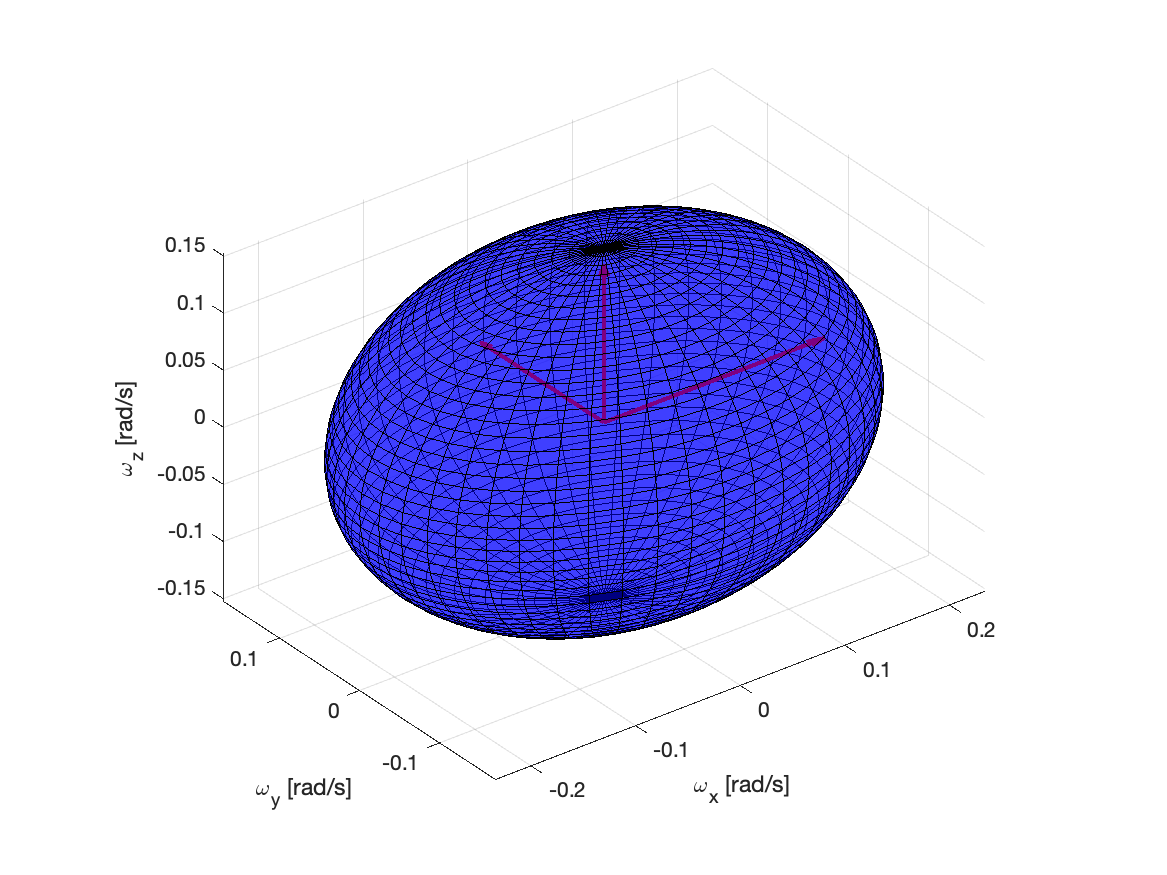
\includegraphics[scale=0.5]{Images/ps2_problem6_energy.png}
\caption{Energy ellipsoid with axes in red}
\label{fig:ps2_problem6_energy}
\end{figure}

\begin{figure}[H]
\centering
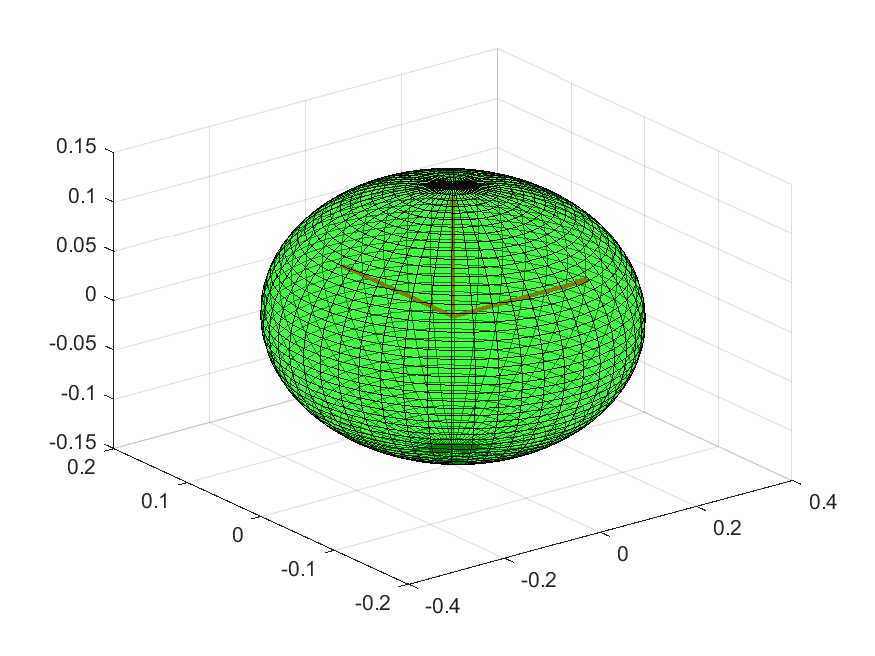
\includegraphics[scale=0.5]{Images/ps2_problem6_momentum.png}
\caption{Momentum ellipsoid with axes in red}
\label{fig:ps2_problem6_momentum}
\end{figure}


\subsection{PROBLEM 7}
\textit{Plot polhode in same 3D plot. Verify that it is the intersection between the ellipsoids.}

For a polhode plot to be real, the condition below must be verified.

\begin{equation*}
    I_x < \frac{L^2}{2T} < I_z
\end{equation*}

Based on previously calculated values ($I_x = 7707.1$, $\frac{L^2}{2T} = 13752.1$, $I_z = 18050.4$) we can verify that the polhode here will be real.

Figure \ref{fig:ps2_problem8} shows that the polhode is indeed the intersection between the ellipsoids.

\begin{figure}[H]
\centering
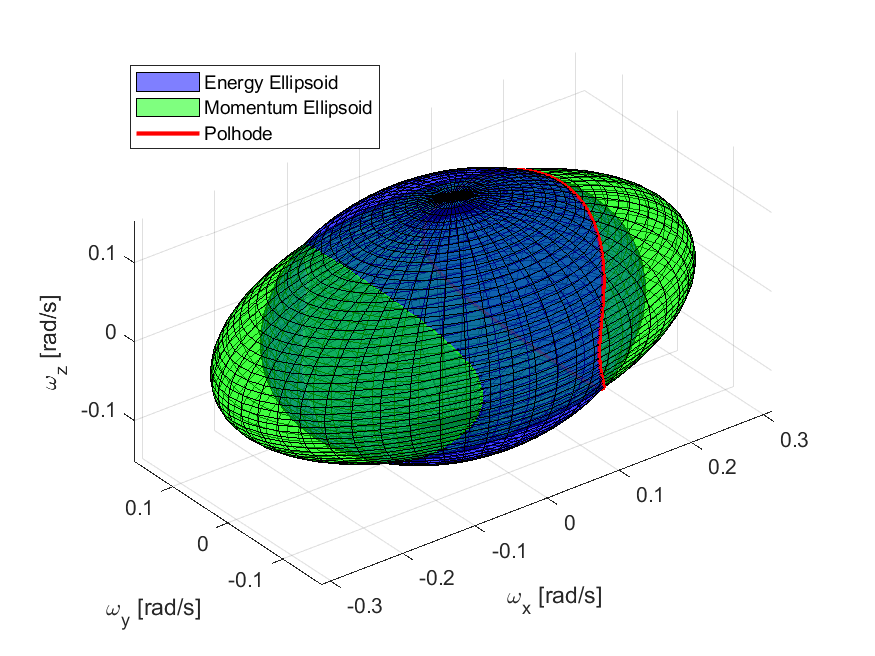
\includegraphics[scale=0.65]{Images/ps2_problem7.png}
\caption{Energy and momentum ellipsoids with polhode}
\label{fig:ps2_problem7}
\end{figure}

\subsection{PROBLEM 8}
\textit{Plot polhode in three 2D planes identified by principal axes (axis equal). Verify that shapes of resulting conic sections correspond to theory.}

The polhode conic sections in Figure \ref{fig:ps2_problem8} match expected theory. The polhode as seen along the x-axis is an ellipse, while the polhode along the y-axis is a hyperbola. We also see that when seen along the z-axis, the polhode also forms an ellipse, shown as a half-ellipse in our plot.

\begin{figure}[H]
\centering
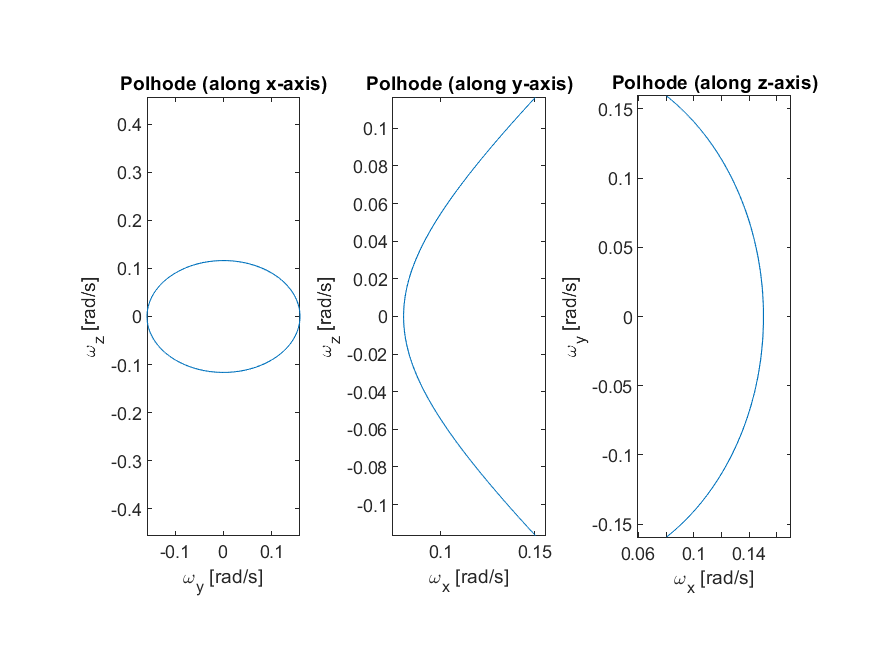
\includegraphics[scale=0.7]{Images/ps2_problem8.png}
\caption{2D views of polhode}
\label{fig:ps2_problem8}
\end{figure}


\subsection{PROBLEM 9}
\textit{Repeat above steps changing initial conditions, e.g. setting angular velocity vector parallel to principal axis. Is the behavior according to expectations?}

We show the angular velocity evolution with the initial conditions shown in Table \ref{tab:ps2_problem9_conditions}. Case 1 involves rotation about the principal x-axis, Case 2 involves rotation about the principal y-axis with a slight disturbance, and Case 3 involved rotation about the z-axis with a slight disturbance.

\begin{table}[H]
\centering
\label{tab:ps2_problem9_conditions}
\begin{tabular}{|l|l|l|l|}
\hline
\textbf{Case} & \textbf{$\omega_x$ (deg/s)} & \textbf{$\omega_y$ (deg/s)} & \textbf{$\omega_z$ (deg/s)} \\ \hline
1             & 8                     & 0                     & 0                     \\ \hline
2             & 0.08                  & 8                     & 0.08                  \\ \hline
3             & 0.08                  & 0                     & 8                     \\ \hline
\end{tabular}
\end{table}

The specifics of Case 1 are shown in the angular velocity plot in Figure \ref{fig:ps2_problem9_euler_equations_x}, the polhode and ellipsoids in Figure \ref{fig:ps2_problem9_p7_x}, and the 2D views of the polhode in Figure \ref{fig:ps2_problem9_p8_x}. The behavior shown is as expected–when the angular velocity is parallel to the principal axis, we do not have coupling with the other components of angular velocity, and the polhode views in 2D become points rather than conic sections.

For Case 2, Figure \ref{fig:ps2_problem9_euler_equations_y} shows that the satellite's rotational behavior will oscillate as expected, owing to the properties of the intermediate axis. Additionally, Figure \ref{fig:ps2_problem9_p7_y}, and the 2D views in Figure \ref{fig:ps2_problem9_p8_y} show a larger polhode, with the slight disturbances leading to ellipsoids with a substantial intersection. Interestingly, there seems to be a very sharp hyperbola in the xz-plane of the polhode.

Figure \ref{fig:ps2_problem9_euler_equations_z} illustrates a slight oscillation of angular velocities about the x- and y-axes in Case 3. Meanwhile, the actual region of intersection in the polhode as shown in Figures \ref{fig:ps2_problem9_p7_z} and \ref{fig:ps2_problem9_p8_z} is much smaller than in other cases, but not a single point like in the Case 1.

\begin{figure}[H]
\centering
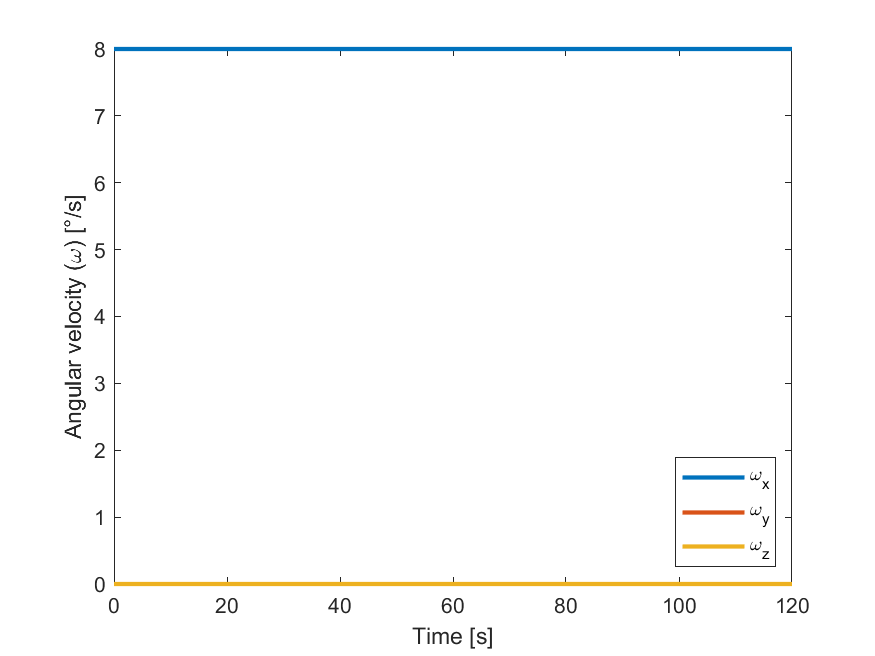
\includegraphics[scale=0.6]{Images/ps2_problem9_euler_equations_x.png}
\caption{Angular velocity evolution for angular velocity vector for Case 1}
\label{fig:ps2_problem9_euler_equations_x}
\end{figure}

\begin{figure}[H]
\centering
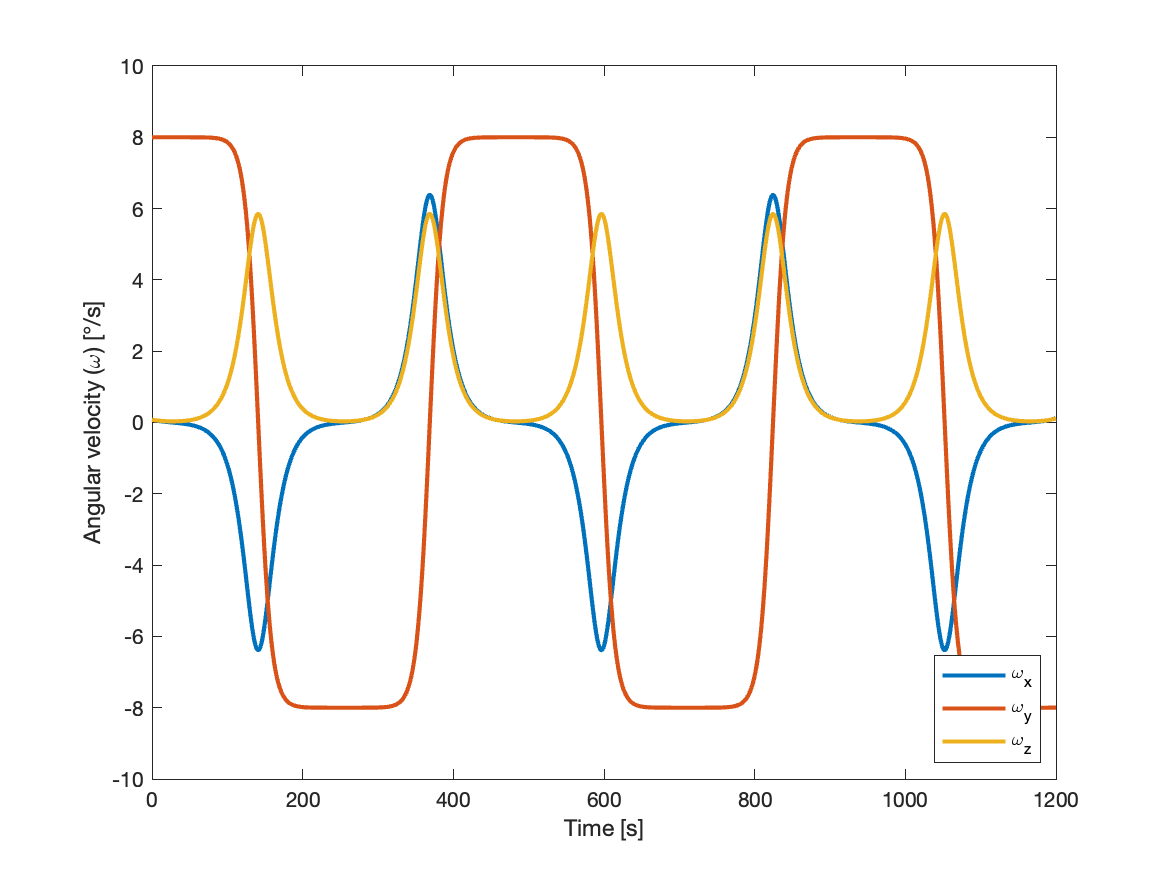
\includegraphics[scale=0.6]{Images/ps2_problem9_euler_equations_y.png}
\caption{Angular velocity evolution for angular velocity vector for Case 2}
\label{fig:ps2_problem9_euler_equations_y}
\end{figure}

\begin{figure}[H]
\centering
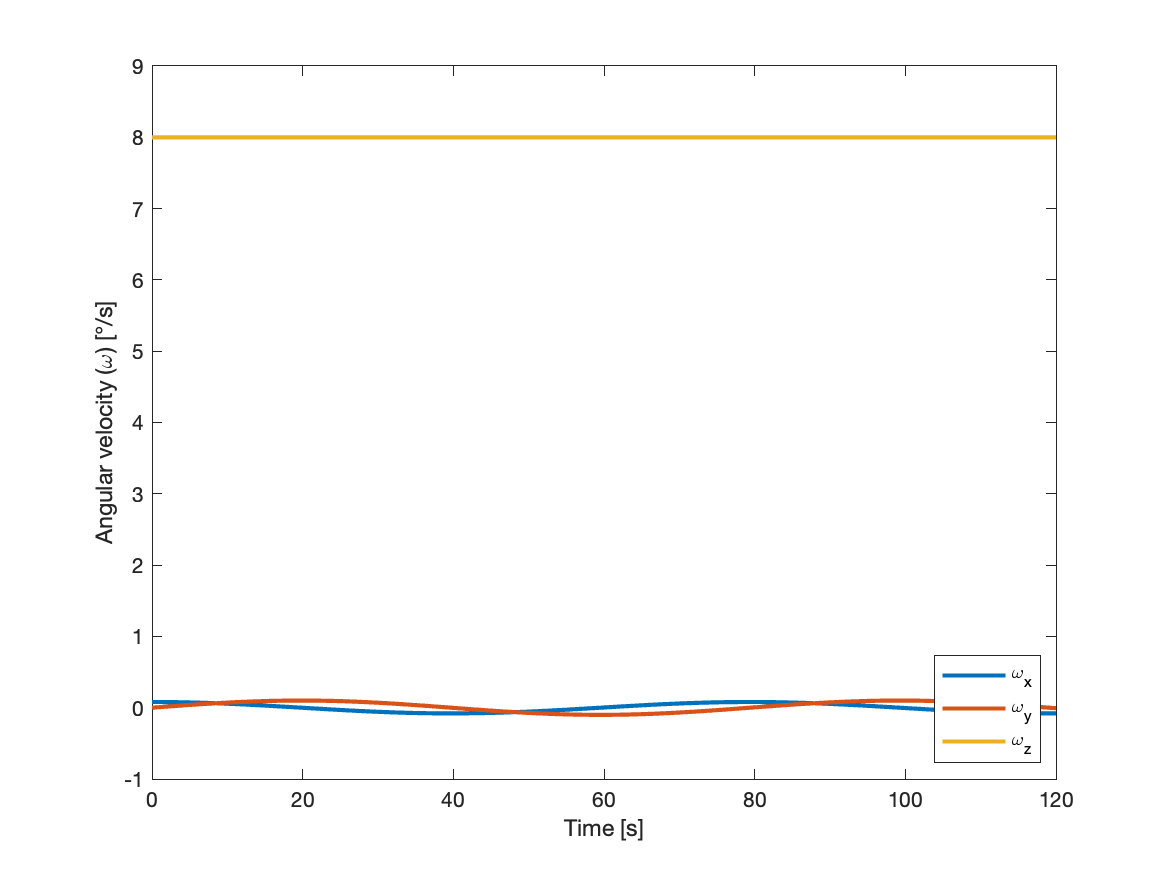
\includegraphics[scale=0.6]{Images/ps2_problem9_euler_equations_z.png}
\caption{Angular velocity evolution for angular velocity vector for Case 3}
\label{fig:ps2_problem9_euler_equations_z}
\end{figure}

\begin{figure}[H]
\centering
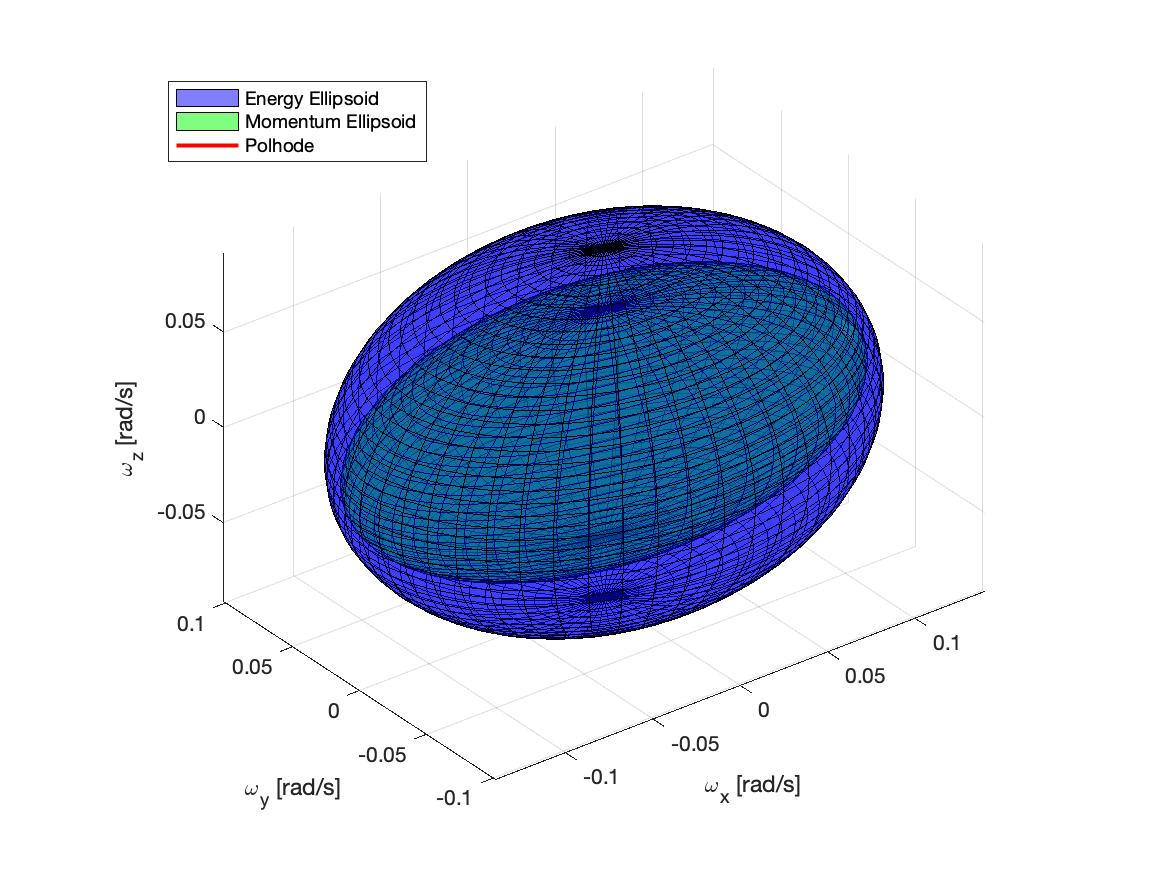
\includegraphics[scale=0.6]{Images/ps2_problem9_p7_x.png}
\caption{Polhode and ellipsoids for angular velocity vector for Case 1}
\label{fig:ps2_problem9_p7_x}
\end{figure}

\begin{figure}[H]
\centering
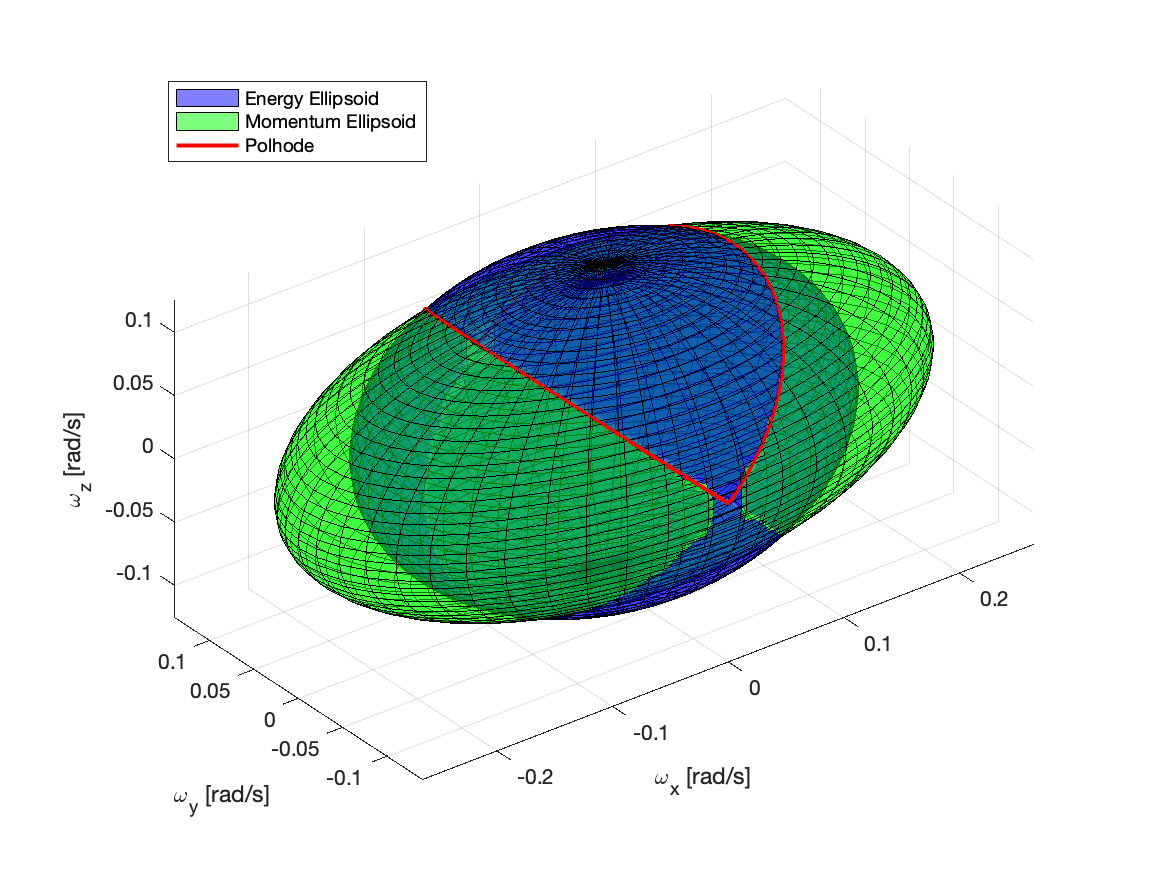
\includegraphics[scale=0.6]{Images/ps2_problem9_p7_y.png}
\caption{Polhode and ellipsoids for angular velocity vector for Case 2}
\label{fig:ps2_problem9_p7_y}
\end{figure}

\begin{figure}[H]
\centering
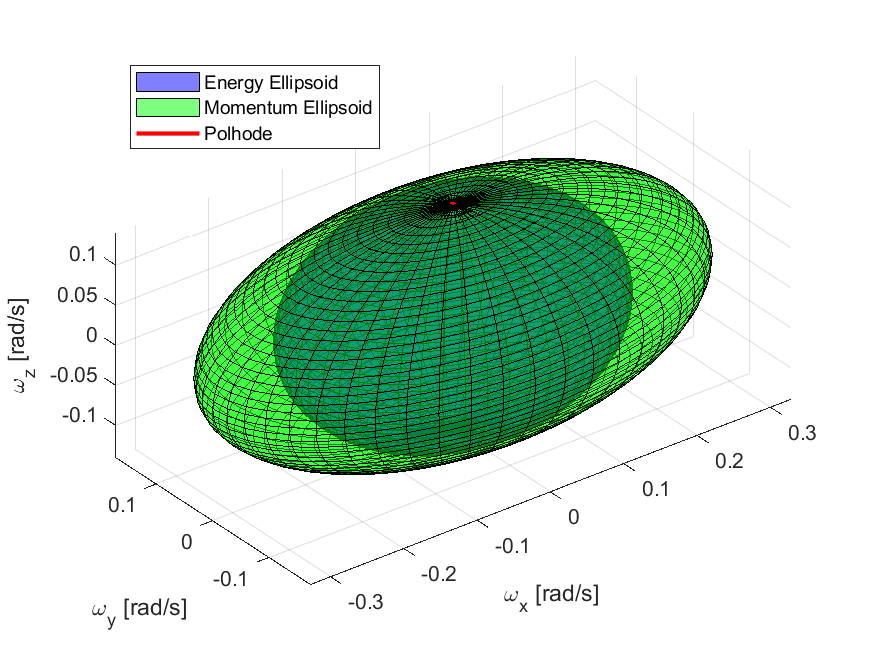
\includegraphics[scale=0.6]{Images/ps2_problem9_p7_z.png}
\caption{Polhode and ellipsoids for angular velocity vector for Case 3}
\label{fig:ps2_problem9_p7_z}
\end{figure}

\begin{figure}[H]
\centering
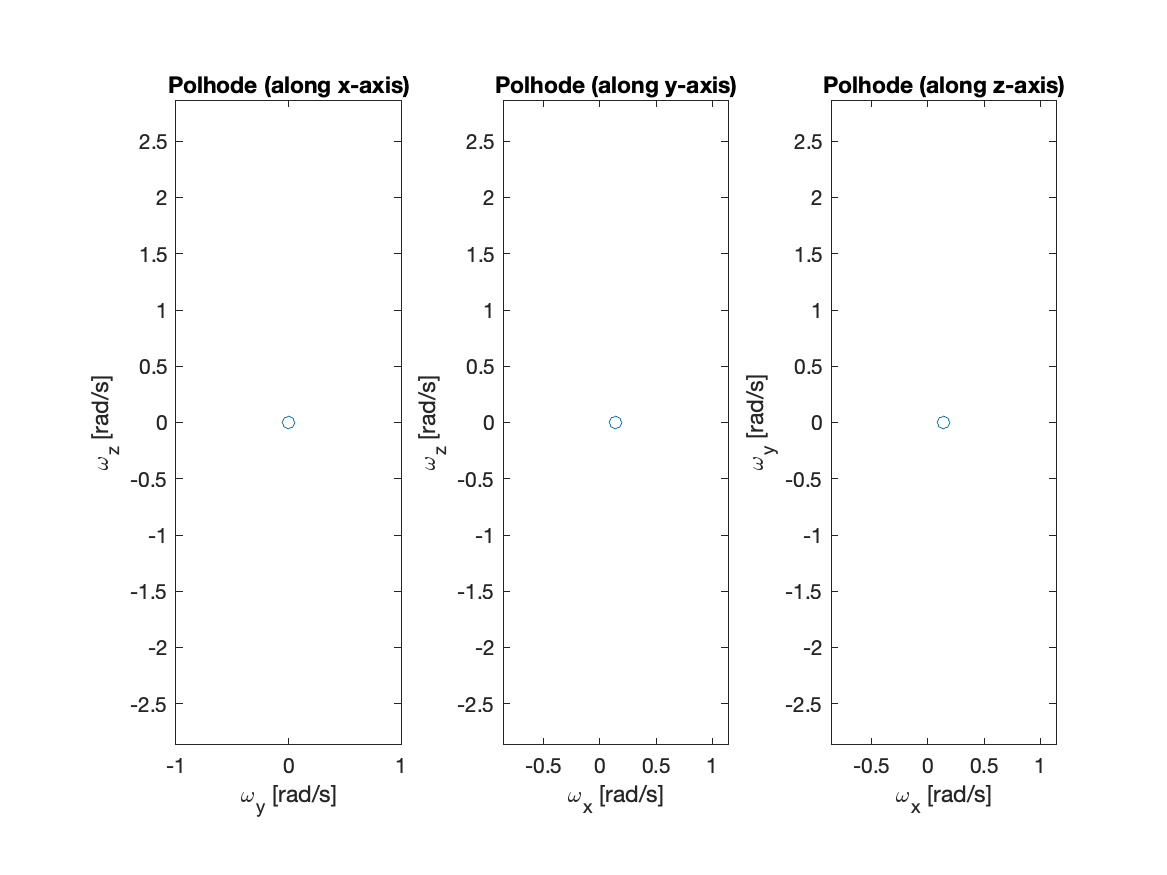
\includegraphics[scale=0.6]{Images/ps2_problem9_p8_x.png}
\caption{2D views of polhode for angular velocity vector for Case 1}
\label{fig:ps2_problem9_p8_x}
\end{figure}

\begin{figure}[H]
\centering
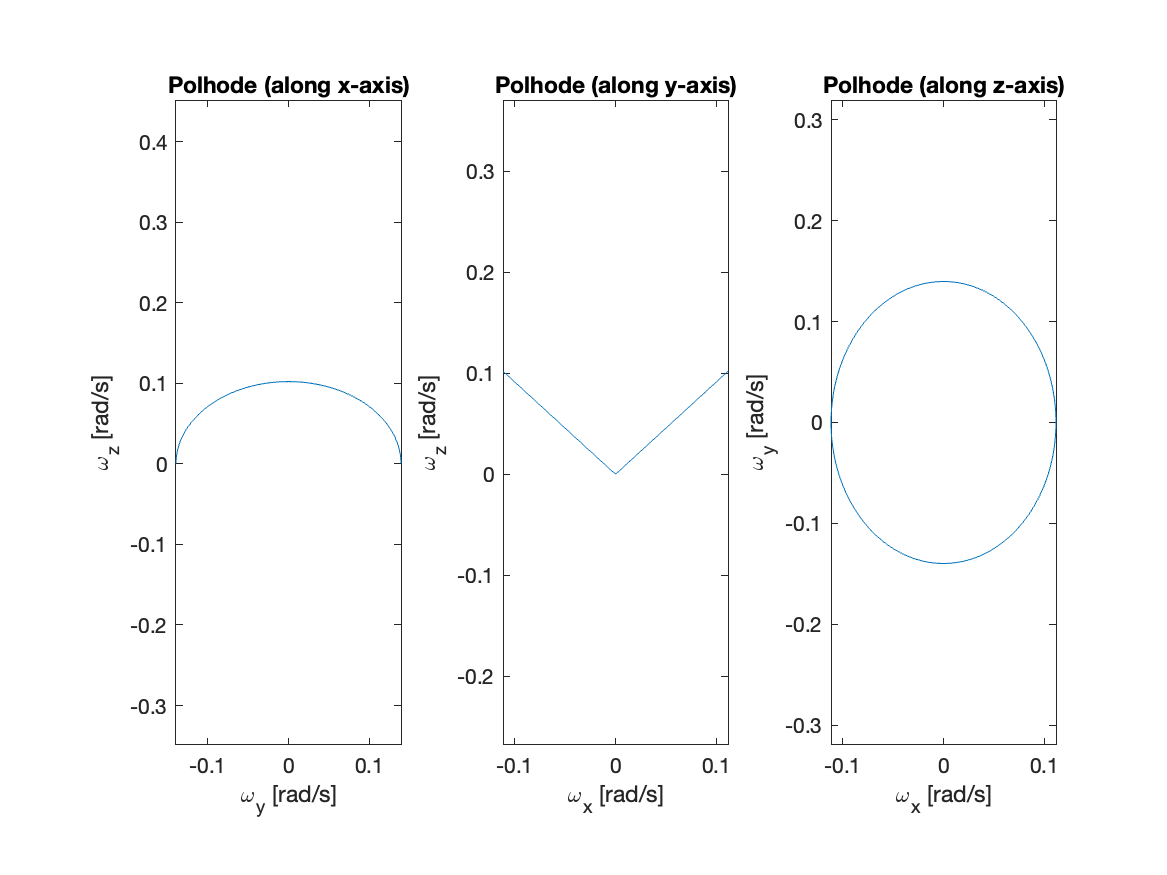
\includegraphics[scale=0.6]{Images/ps2_problem9_p8_y.png}
\caption{2D views of polhode for angular velocity vector for Case 1}
\label{fig:ps2_problem9_p8_y}
\end{figure}

\begin{figure}[H]
\centering
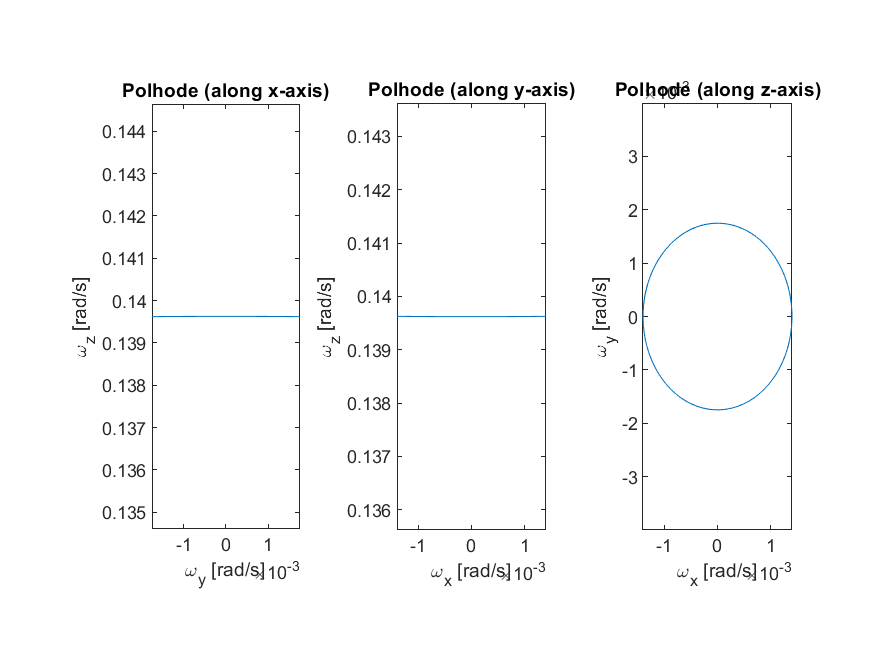
\includegraphics[scale=0.6]{Images/ps2_problem9_p8_z.png}
\caption{2D views of polhode for angular velocity vector for Case 1}
\label{fig:ps2_problem9_p8_z}
\end{figure}